%% Source: https://github.com/tias/constraint-solving-course
%% Licensed under CC BY-NC-SA 4.0: https://creativecommons.org/licenses/by-nc-sa/4.0/
%% You may share and adapt this for non-commercial use,
%% with attribution and under the same license.

\documentclass{cons-beamer}

% custom columns for array package:
\newcolumntype{C}{>{\centering\arraybackslash}p{65mm}} % comb opti examples
\newcolumntype{D}{>{\centering\arraybackslash}p{11mm}} % doctor rostering 
\newcolumntype{G}{>{\centering}m{9mm}} % genotypes
\newcolumntype{H}{>{\centering}m{4mm}} % haplotypes

% commands for BIBD, AED:
\newcommand{\VarSem}{sample}           \newcommand{\BlkSem}{growth}
\newcommand{\Variety}{grain}           \newcommand{\Block}{\textnormal{plot}}
\newcommand{\VarBlk}{grown in}         \newcommand{\BlkVar}{grows}
\newcommand{\BlkVarAlt}{grow}
\newcommand{\VarOne}{barley}           \newcommand{\BlkOne}{\Block1}
\newcommand{\VarTwo}{corn}             \newcommand{\BlkTwo}{\Block2}
\newcommand{\VarThree}{millet}         \newcommand{\BlkThree}{\Block3}
\newcommand{\VarFour}{oats}            \newcommand{\BlkFour}{\Block4}
\newcommand{\VarFive}{rye}             \newcommand{\BlkFive}{\Block5}
\newcommand{\VarSix}{spelt}            \newcommand{\BlkSix}{\Block6}
\newcommand{\VarSeven}{wheat}          \newcommand{\BlkSeven}{\Block7}

% commands for doctor rostering
\newcommand{\appt}{\defined{appt}}
\newcommand{\call}{\search{call}}
\newcommand{\none}{\relaxation{none}}
\newcommand{\oper}{\inference{oper}}

\begin{document}


\begin{frame}{L01: Intro to Model+Solve and Combinatorial Optimisation}
  \begin{center}
    ~ \\
    \includegraphics[height=38mm]{images/CO_examples} \\
    ~ \\
    Prof. Tias Guns and Dr Dimos Tsouros \\[0.5em]
    \includegraphics[width=2cm]{images/kuleuven_CMYK_logo.pdf}
  \end{center}
  
  {\footnotesize 
  Based on slides from Pierre Flener, Uppsala University + slides from Guido Tack \& Chris Beck.}
  % https://pierre-flener.github.io/courses/M4CO/lectures.html
\end{frame}


\begin{frame}
  \begin{example}[From: Steven S. Skiena's The Algorithm Design Manual]
    \small
    Imagine you are a highly-in-
    demand actor, who has been presented with offers to star in n different movie
    projects under development. Each offer comes specified with the first and last day
    of filming. To take the job, you must commit to being available throughout this
    entire period. Thus, you cannot simultaneously accept two jobs whose intervals
    overlap.

    $ $
    
    For an artist such as yourself, the criteria for job acceptance is clear: you want
    to make as much money as possible. Because each of these films pays the same fee
    per film, this implies you seek the largest possible set of jobs (intervals) such that no two of them conflict with each other.

    \begin{table}[h!]
      \centering
      \tiny
      \begin{tabular}{| m{5cm} | m{2cm} | m{2cm} |}
        \hline
        \textbf{Title} & \textbf{Start} & \textbf{End} \\ \hline
        Tarjan of the Jungle & 4 & 13 \\ \hline
        The Four Volume Problem & 17 & 27 \\ \hline
        The President's Algorist & 1 & 10 \\ \hline
        Steiner's Tree & 12 & 18 \\ \hline
        Process Terminated & 23 & 30 \\ \hline
        Halting State & 9 & 16 \\ \hline
        Programming Challenges & 19 & 25 \\ \hline
        Discrete Mathematics & 2 & 7 \\ \hline
        Calculated Bets & 26 & 31 \\ \hline
      \end{tabular}
    \end{table}
  \end{example}
  How would you solve this problem?
\end{frame}

\begin{frame}
  \begin{example}[From: Steven S. Skiena's The Algorithm Design Manual]
    \small
    Imagine you are a highly-in-
    demand actor, who has been presented with offers to star in n different movie
    projects under development. Each offer comes specified with the first and last day
    of filming. To take the job, you must commit to being available throughout this
    entire period. Thus, you cannot simultaneously accept two jobs whose intervals
    overlap.

    $ $
    
    For an artist such as yourself, the criteria for job acceptance is clear: you want
    to make as much money as possible. Because each of these films pays the same fee
    per film, this implies you seek the largest possible set of jobs (intervals) such that no two of them conflict with each other.

    \begin{table}[h!]
      \centering
      \tiny
      \begin{tabular}{| m{5cm} | m{2cm} | m{2cm} |}
        \hline
        \textbf{Title} & \textbf{Start} & \textbf{End} \\
        \hline
        ... & ... & ... \\
        \hline
      \end{tabular}
    \end{table}
  \end{example}
  How would you solve this problem?
  \begin{enumerate}
    \item Trial and error on paper
    \item Write a custom search algorithm
    \item Reuse an existing, generic problem solving paradigm \alt<2>{\textbf{$\Leftarrow$ This Course}}{}
  \end{enumerate}
\end{frame}

% based on slide from Chris Beck 
\begin{frame}{Model-and-Solve}
  \centering
  \includegraphics[height=68mm]{images/prob2def}
\end{frame}
\begin{frame}{Model-and-Solve}
  \centering
  \includegraphics[height=68mm]{images/prob2sol}
\end{frame}

\begin{frame}{Outline}
  \tableofcontents
\end{frame}

\section{Combinatorial Optimisation Problems}

\begin{frame}{Combinatorial Optimisation}
  \begin{center}
    ~ \\
    \includegraphics[height=48mm]{images/CO_examples} \\
    ~ \\
    \visible<2>{Combinatorial Optimisation is a science of \alert{service}: \\
    to scientists, to engineers, to artists, and to society.}
  \end{center}
\end{frame}

\begin{frame}
  \begin{example}[Agricultural experiment design]
    \begin{table} \small
      \begin{tabular}{r|c|c|c|c|c|c|c|}
        \multicolumn{1}{r}{} & \multicolumn{1}{c}{\BlkOne}
        & \multicolumn{1}{c}{\BlkTwo} & \multicolumn{1}{c}{\BlkThree}
        & \multicolumn{1}{c}{\BlkFour} & \multicolumn{1}{c}{\BlkFive}
        & \multicolumn{1}{c}{\BlkSix} & \multicolumn{1}{c}{\BlkSeven} \\
        \cline{2-8}
        \VarOne   & \alt<2>{\tick}{} & \alt<2>{\tick}{} & \alt<2>{\tick}{} & \alt<2>{--}{} & \alt<2>{--}{} & \alt<2>{--}{} & \alt<2>{--}{} \\ \cline{2-8}
        \VarTwo   & \alt<2>{\tick}{} & \alt<2>{--}{} & \alt<2>{--}{} & \alt<2>{\tick}{} & \alt<2>{\tick}{} & \alt<2>{--}{} & \alt<2>{--}{} \\ \cline{2-8}
        \VarThree & \alt<2>{\tick}{} & \alt<2>{--}{} & \alt<2>{--}{} & \alt<2>{--}{} & \alt<2>{--}{} & \alt<2>{\tick}{} & \alt<2>{\tick}{} \\ \cline{2-8}
        \VarFour  & \alt<2>{--}{} & \alt<2>{\tick}{} & \alt<2>{--}{} & \alt<2>{\tick}{} & \alt<2>{--}{} & \alt<2>{\tick}{} & \alt<2>{--}{} \\ \cline{2-8}
        \VarFive  & \alt<2>{--}{} & \alt<2>{\tick}{} & \alt<2>{--}{} & \alt<2>{--}{} & \alt<2>{\tick}{} & \alt<2>{--}{} & \alt<2>{\tick}{} \\ \cline{2-8}
        \VarSix   & \alt<2>{--}{} & \alt<2>{--}{} & \alt<2>{\tick}{} & \alt<2>{\tick}{} & \alt<2>{--}{} & \alt<2>{--}{} & \alt<2>{\tick}{} \\ \cline{2-8}
        \VarSeven & \alt<2>{--}{} & \alt<2>{--}{} & \alt<2>{\tick}{} & \alt<2>{--}{} & \alt<2>{\tick}{} & \alt<2>{\tick}{} & \alt<2>{--}{} \\
        \cline{2-8}
      \end{tabular}
    \end{table}
    \textbf{Constraints} to be \textbf{satisfied}:
    \begin{enumerate}
      \item Equal \VarSem\ size: Every \Variety\ is \VarBlk\ 3 \Block s.
      \item Equal \BlkSem\ load: Every \Block\ \BlkVar\ 3 \Variety s.
      \item Balance: Every \Variety\ pair is \VarBlk\ 1 common \Block.
    \end{enumerate}
    \textbf{Instance}: $7$ \Block s, $7$ \Variety s, $3$ \Variety
    s/\Block, $3$ \Block s/\Variety, balance~$1$.
  \end{example}
\end{frame}

\begin{frame}
  \begin{example}[Doctor rostering]
    \begin{table}
      \begin{tabular}{l|D|D|D|D|D|D|D|}
        \multicolumn{1}{l}{} & \multicolumn{1}{c}{Mon} & \multicolumn{1}{c}{Tue} & \multicolumn{1}{c}{Wed} & \multicolumn{1}{c}{Thu} & \multicolumn{1}{c}{Fri} & \multicolumn{1}{c}{Sat} & \multicolumn{1}{c}{Sun} \\
        \cline{2-8}
        Doctor A & \alt<2>{\call}{} & \alt<2>{\none}{} & \alt<2>{\oper}{} & \alt<2>{\none}{} & \alt<2>{\oper}{} & \alt<2>{\none}{} & \alt<2>{\none}{} \\ \cline{2-8}
        Doctor B & \alt<2>{\appt}{} & \alt<2>{\call}{} & \alt<2>{\none}{} & \alt<2>{\oper}{} & \alt<2>{\none}{} & \alt<2>{\none}{} & \alt<2>{\call}{} \\ \cline{2-8}
        Doctor C & \alt<2>{\oper}{} & \alt<2>{\none}{} & \alt<2>{\call}{} & \alt<2>{\appt}{} & \alt<2>{\appt}{} & \alt<2>{\call}{} & \alt<2>{\none}{} \\ \cline{2-8}
        Doctor D & \alt<2>{\appt}{} & \alt<2>{\oper}{} & \alt<2>{\none}{} & \alt<2>{\call}{} & \alt<2>{\oper}{} & \alt<2>{\none}{} & \alt<2>{\none}{} \\ \cline{2-8}
        Doctor E & \alt<2>{\oper}{} & \alt<2>{\none}{} & \alt<2>{\oper}{} & \alt<2>{\none}{} & \alt<2>{\call}{} & \alt<2>{\none}{} & \alt<2>{\none}{} \\ \cline{2-8}
      \end{tabular}
    \end{table}\vspace{-7pt}
    \textbf{Constraints} to be \textbf{satisfied}: \\[+5pt]
    \vfill
    \begin{minipage}[c]{0.49\textwidth}
      \begin{enumerate}
      \item \#\search{on-call doctors} / day $=$ 1
      \item \#\inference{operating doctors} / weekday $\leq$ 2
      \item \#\inference{operating doctors} / week $\geq$ 7
      \item \#\defined{appointed doctors} / week $\geq$ 4
      \item \relaxation{day off} after \inference{operation day}
      \item \dots
      \end{enumerate}
    \end{minipage}
    \hfill
    \begin{minipage}[c]{0.50\textwidth}
      \visible<2>{\includegraphics[width=63mm]{images/physicians}}
    \end{minipage} \\[+5pt]
    \textbf{Objective function} to be \textbf{minimised}:
    Cost: \dots
  \end{example}
\end{frame}

\begin{frame}
  \begin{example}[Vehicle routing: parcel delivery]
    \structured{Given} a depot with parcels for clients and a vehicle
    fleet, \\ \structured{find} which vehicle visits which client when. 
    \\ [+1mm]

    \textbf{Constraints} to be \textbf{satisfied}: \\
    \begin{minipage}[c]{0.59\textwidth}
      \begin{enumerate}
        \item All parcels are delivered on time. \vfill
        \item No vehicle is overloaded. \vfill
        \item Driver regulations are respected. \vfill
        \item \dots
      \end{enumerate}
    \end{minipage}
    \hfill
    \begin{minipage}[c]{0.40\textwidth}
      \includegraphics[width=40mm]{images/VRP}
    \end{minipage} \vfill
    \textbf{Objective function} to be \textbf{minimised}:
    \begin{itemize}
      \item Cost: the total fuel consumption and driver salary.
    \end{itemize}
  \end{example}\vfill

  \begin{example}[Travelling salesperson: optimisation TSP]
    \structured{Given} a map and cities, \\ \structured{find} a
    \textbf{shortest} route visiting each city once and returning to
    the starting city.
  \end{example}
\end{frame}

\begin{frame}{Applications in Air Traffic Management}
  \begin{tabular}{CC}
    \structured{Demand vs capacity} \newline
    \includegraphics[height=25mm]{images/routes}
    &
    \structured{Airspace sectorisation} \newline
    \includegraphics[height=25mm]{images/sectorLondon}    
    \\[+8mm]
    \structured{Contingency planning} \newline\newline
    \tiny
    \begin{tabular}{|l|c|c|}
      \hline
      Flow & Time Span & Hourly Rate \\
      \hline
      From: Arlanda   & 00:00 -- 09:00 & 3 \\
      To: west, south & 09:00 -- 18:00 & 5 \\
                      & 18:00 -- 24:00 & 2 \\
      \hline
      From: Arlanda   & 00:00 -- 12:00 & 4 \\
      To: east, north & 12:00 -- 24:00 & 3 \\
      \hline
      \dots & \dots & \dots \\
      \hline
    \end{tabular}
    &
    \structured{Workload balancing} \newline
    \includegraphics[height=25mm]{images/atm}
  \end{tabular}
\end{frame}

\begin{frame}
  \begin{example}[Air-traffic demand-capacity balancing]
    Reroute flights, in height and speed, so as to balance the
    workload of air traffic controllers in a multi-sector airspace:
    \vfill
    \begin{center}
      \includegraphics[height=58mm]{images/routes}
    \end{center}
  \end{example}
\end{frame}

\begin{frame}
  \begin{example}[Airspace sectorisation]
    \begin{tabular}{p{60mm}p{60mm}}
      \structured{Given} an airspace split into $c$ cells,
      a targeted number $s$ of sectors, and~flight schedules. &
      \structured{Find} a colouring of the $c$ cells into~$s$
      connected convex sectors, with minimal imbalance of the
      workloads of their air traffic controllers. \\
      \includegraphics[height=40mm]{images/hexLondon} \hfill & 
      \includegraphics[height=40mm]{images/sectorLondon}
    \end{tabular}
    \\ There are $s^c$ possible colourings, but very few optimally
    satisfy the constraints: is \alert{intelligent} search necessary?
  \end{example}
\end{frame}

\begin{frame}{Applications in Biology and Medicine}
  \begin{tabular}{CC}
    \structured{Phylogenetic supertree} \newline
    \includegraphics[height=28mm]{images/seabirds}
    &
    \structured{Haplotype inference} \newline
    \includegraphics[height=25mm]{images/genotype-haplotype}
    \\[+8mm]
    \structured{Medical image analysis} \newline
    \includegraphics[width=50mm]{images/medical}
    &
    \structured{Doctor rostering}\invisible{gy} \newline
    \includegraphics[width=50mm]{images/physicians}
  \end{tabular}
\end{frame}

\begin{frame}
  \begin{example}[Given several phylogentic trees, what supertree is maximally consistent with shared species in the trees?]
    \centering
    \includegraphics[width=100mm]{images/seabirds.pdf}
  \end{example}
\end{frame}

\begin{frame}
  \begin{example}[Haplotype inference by pure parsimony]
    \structured{Given} $n$ child genotypes, with homo- and
    heterozygous sites:
    \begin{center} \footnotesize
      \begin{tabular}{|G|G|G|G|G|G|}
        \hline
        \multicolumn{6}{|c|}{$\cdots$} \tabularnewline \hline
        A & \blue{C} / \red{G} & T & C & \blue{A} / \red{T} & C \tabularnewline \hline
        \multicolumn{6}{|c|}{$\cdots$} \tabularnewline \hline
        A / T & G & T & C / G & A & C  \tabularnewline \hline
        \multicolumn{6}{|c|}{$\cdots$} \tabularnewline \hline
      \end{tabular}
    \end{center}
    \structured{find} a minimal set of (at most $2 \cdot n$) parent
    haplotypes:
    \begin{center} \footnotesize
      \begin{tabular}{|c|c|c|c|c|c|}
        \hline
        \multicolumn{6}{|c|}{$\cdots$} \\ \hline
        A & \blue{C} & T & C & \red{T} & C \\ \hline
        \multicolumn{6}{|c|}{$\cdots$} \\ \hline
        A & \red{G} & T & C & \blue{A} & C \\ \hline
        \multicolumn{6}{|c|}{$\cdots$} \\ \hline
        T & G & T & G & A & C          \\ \hline
        \multicolumn{6}{|c|}{$\cdots$} \\ \hline
      \end{tabular}
    \end{center}
    \structured{so that} each given genotype conflates (is the merge of) 2 found
    haplotypes.
  \end{example}
\end{frame}

\begin{frame}{Applications in Programming and Testing}
  \begin{tabular}{CC}
    \structured{Robot programming} \newline
    \includegraphics[width=50mm]{images/ABB-FRIDA}
    &
    \structured{Sensor-net configuration} \newline
    \includegraphics[width=50mm]{images/WSN}
    \\[+8mm]
    \structured{Compiler design} \newline
    \includegraphics[height=30mm]{images/instruction-scheduling}
    &
    \structured{Base-station testing}
    \includegraphics[height=30mm]{images/baseStation}
  \end{tabular}
\end{frame}

\begin{frame}{Other Application Areas}
  \begin{tabular}{CC}
    \structured{School timetabling} \newline
    \includegraphics[height=30mm]{images/timetable}
    &
    \structured{Sports tournament design} \newline
    \includegraphics[height=5mm]{images/SEH} \newline
    \includegraphics[height=25mm]{images/handball}
    \\[+8mm]
    \structured{Security: SQL injection} \newline
    \includegraphics[height=24mm]{images/sqlinjection.png}
    &
    \structured{Container packing} \newline
    \includegraphics[height=27mm]{images/binPacking}
    % &
    % \structured{Financial designs} \newline
    % \includegraphics[height=27mm]{images/WallStreet}
  \end{tabular}
\end{frame}


\section{Search and constraint solving paradigms}

\begin{frame}
  Let's reconsider: 
  \begin{example}[Agricultural experiment design]
    \begin{table} \small
      \begin{tabular}{r|c|c|c|c|c|c|c|}
        \multicolumn{1}{r}{} & \multicolumn{1}{c}{\BlkOne}
        & \multicolumn{1}{c}{\BlkTwo} & \multicolumn{1}{c}{\BlkThree}
        & \multicolumn{1}{c}{\BlkFour} & \multicolumn{1}{c}{\BlkFive}
        & \multicolumn{1}{c}{\BlkSix} & \multicolumn{1}{c}{\BlkSeven} \\
        \cline{2-8}
        \VarOne   & {\tick}{} & {\tick}{} & {\tick}{} & {--}{} & {--}{} & {--}{} & {--}{} \\ \cline{2-8}
        \VarTwo   & {\tick}{} & {--}{} & {--}{} & {\tick}{} & {\tick}{} & {--}{} & {--}{} \\ \cline{2-8}
        \VarThree & {\tick}{} & {--}{} & {--}{} & {--}{} & {--}{} & {\tick}{} & {\tick}{} \\ \cline{2-8}
        \VarFour  & {--}{} & {\tick}{} & {--}{} & {\tick}{} & {--}{} & {\tick}{} & {--}{} \\ \cline{2-8}
        \VarFive  & {--}{} & {\tick}{} & {--}{} & {--}{} & {\tick}{} & {--}{} & {\tick}{} \\ \cline{2-8}
        \VarSix   & {--}{} & {--}{} & {\tick}{} & {\tick}{} & {--}{} & {--}{} & {\tick}{} \\ \cline{2-8}
        \VarSeven & {--}{} & {--}{} & {\tick}{} & {--}{} & {\tick}{} & {\tick}{} & {--}{} \\

        \cline{2-8}
      \end{tabular}
    \end{table}
    \textbf{Constraints} to be \textbf{satisfied}:
    \begin{enumerate}
      \item Equal \VarSem\ size: Every \Variety\ is \VarBlk\ 3 \Block s.
      \item Equal \BlkSem\ load: Every \Block\ \BlkVar\ 3 \Variety s.
      \item Balance: Every \Variety\ pair is \VarBlk\ 1 common \Block.
    \end{enumerate}
    \textbf{Instance}: $7$ \Block s, $7$ \Variety s, $3$ \Variety
    s/\Block, $3$ \Block s/\Variety, balance~$1$.
  \end{example}

  Could you compute a solution for 50 grains and 20 plots? for 1000 grains?
\end{frame}

\begin{frame}{P $\overset{?}{=}$ NP \hfill (Cook, 1971; Levin, 1973)}
  This is one of the seven
  \href{https://www.claymath.org/millennium/p-vs-np}{Millennium Prize}
  problems of the Clay Mathematics Institute (Massachusetts, USA),
  each worth 1~million~US\$. \vfill
  
  Informally:
  \begin{itemize}
    \item P = class of problems that need \alert{no} search to be solved \\
      NP = class of problems that \alert{might} need search to solve 
    \item P = class of problems with easy-to-\alert{compute} solutions \\
      NP = class of problems with easy-to-\alert{check} solutions
  \end{itemize}
  Thus: Can search always be avoided (P $=$ NP), \\ or is search
  sometimes necessary (P $\neq$ NP)? \vfill

  Problems that are solvable in polynomial time (in the input size)
  are considered \defined{tractable}, aka \defined{easy}. \\ Problems
  needing super-polynomial time are considered \defined{intractable},
  aka \defined{hard}.
\end{frame}

\begin{frame}[label={longest}]{NP Completeness: Examples}
  Given a digraph $(V,E)$:
  \begin{examples}
    \begin{itemize}
    \item Finding a \defined{shortest path} takes 
      $\Oh{V \cdot E}$ time and is thus in P. 
    \item Determining the existence of a simple path (which has
      distinct vertices), from a given single source, that has
      \emph{at least} a given number $\ell$ of edges \\ is
      NP-complete.  Hence finding a \defined{longest path}
      seems hard: \\ increase $\ell$ starting from a trivial lower
      bound, until answer is `no'.
    \end{itemize}
  \end{examples} 
  \begin{examples}
    \begin{itemize}
    \item Finding an \defined{Euler tour} (which visits each
      \emph{edge} once) takes  $\Oh{E}$ time \\ and is thus in P. 
    \item Determining the existence of a \defined{Hamiltonian cycle}
      (which visits each \emph{vertex} once) is NP-complete.
    \end{itemize}
  \end{examples}
\end{frame}

\begin{frame}{NP Completeness: More Examples}
  \begin{examples}
    \begin{itemize}
      \item \defined{$n$-SAT}: Determining the satisfiability of a
        conjunction of disjunctions of~$n$~Boolean literals is in P for
        $n=2$  but NP-complete for $n=3$. 
      \item \defined{SAT}: Determining the satisfiability of a formula
        over Boolean literals is NP-complete. 
      \item \defined{Clique}: Determining the existence of a clique
        (complete subgraph) of a given size in a graph is NP-complete.
        
      \item \defined{Vertex Cover}: Determining the existence of a
        vertex cover (a vertex subset with at least one endpoint for all
        edges) of a given size in a graph is NP-complete. 
      \item \defined{Subset Sum}: Determining the existence of a subset,
        of a given set, that has a given sum is NP-complete.
    \end{itemize}
  \end{examples}
\end{frame}

\begin{frame}
  Search spaces are often larger than the universe! \vfill
  \includegraphics[height=50mm]{images/burningLaptop} \\
  Many important real-life problems are NP-hard or worse: their
  real-life instances can only be solved exactly and fast enough by
  \alert{intelligent} search, unless $\text{P} =
  \text{NP}$. 
  
  $ $ \\
  \alert{NP-hardness is not where the fun ends, its where it begins!}
\end{frame}

\begin{frame}
  \begin{example}[Optimisation TSP over $n$ cities]
    A brute-force algorithm evaluates all $n!$ candidate routes:
    \begin{itemize}
    \item A computer of today evaluates $10^6$ routes / second:
      \begin{center}\footnotesize
        \begin{tabular}{lr}
          $n$ & time \\
          \hline
          $11$  & $40$ seconds \\ 
          $14$  & $1$ day \\ 
          $18$  & $203$ years \\ 
          $20$  & $77$k years
        \end{tabular}
      \end{center}
    \item Planck time is shortest useful interval:
      $\approx 5.4 \cdot 10^{-44}$~second; \\ a Planck computer would
      evaluate $1.8 \cdot 10^{43}$ routes / second: 
      \begin{center}\footnotesize
        \begin{tabular}{lr}
          $n$ & time \\
          \hline
          $37$  & $0.7$ seconds \\ 
          $41$  & $20$ days \\ 
          $48$  & $1.5 ~\cdot$ age of universe
        \end{tabular}
      \end{center}
    \end{itemize}
    The \underline{dynamic program} by Bellman-Held-Karp ``only'' takes
    $\Oh{n^2 \cdot 2^n}$ time: \\ a computer of today takes a day for
    $n=27$, a year for $n=35$, the age of the universe for $n=67$, and
    beats the $\Oh{n!}$ algo on
    Planck computer for $n \geq 44$.
  \end{example}
\end{frame}

\begin{frame}{Intelligent Search upon NP-Hardness}
  \alert{Do not give up but try to stay ahead of the curve: \\ there
    is an instance size until which an \textbf{exact} algorithm is
    fast enough!}
  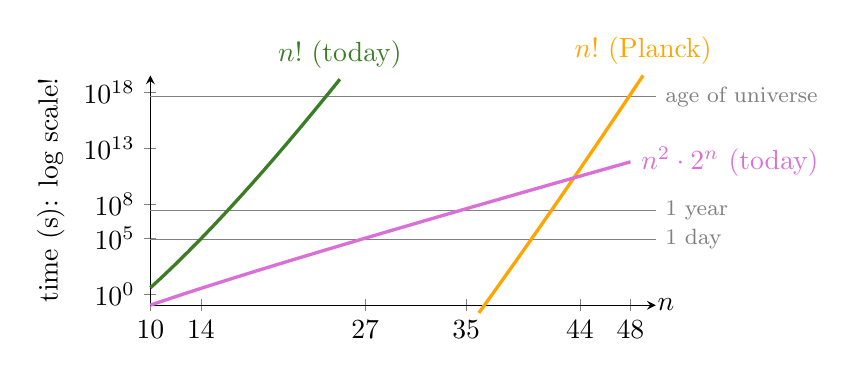
\begin{tikzpicture} \centering
    \begin{semilogyaxis}[height=45mm, width=8cm, clip=false, axis lines=left,
      xlabel={$n$}, x label style={at={(1.02,0.07)}},
      xmin=10, xmax=50, xtick={10,14,27,35,44,48},
      ylabel={time (s): log scale!},
      ymin=0.1, ytickten={0,5,8,13,18}]
      \draw[very thin,color=gray] (10,86400) -- (50,86400)
        node[right] {\footnotesize 1 day};
      \draw[very thin,color=gray] (10,31536000) -- (50,31536000)
        node[right] {\footnotesize 1 year};
      \draw[very thin,color=gray] (10,4.35*10^17) -- (50,4.35*10^17)
        node[right] {\footnotesize age of universe}; % 13.8 billion years
      \addplot[OliveGreen,very thick,domain=10:25,samples=16] {x!/(10^6)}
        node[above] {$n!$ (today)};
      \addplot[Orange,very thick,domain=36:49,samples=14] {x!/(1.8*10^43)}
        node[above] {$n!$ (Planck)};
      \addplot[Orchid,very thick,domain=10:48,samples=39] {(x^2)*(2^x)/(10^6)}
        node[right] {$n^2 \cdot 2^n$ (today)};
    \end{semilogyaxis}
  \end{tikzpicture}  \\
  \href{https://www.math.uwaterloo.ca/tsp/concorde}{Concorde TSP Solver} beats the
  \defined{Bellman-Held-Karp} exact algo: it uses local search \&
  approximation algos, but sometimes proves exactness of its optima.
  The largest instance solved exactly, in $136$ CPU years in 2006, has $n=85900$.
\end{frame}

\begin{frame}
  A \defined{declarative problem solving paradigm} offers languages, methods, and tools for: \vfill
  \begin{itemize}
    \item[what:] \textbf{Modelling} combinatorial problems in a \alert{declarative} language.
  \end{itemize}\vfill
  and / or \vfill
  \begin{itemize}
    \item[how:] \textbf{Solving} combinatorial problems \inference{intelli}\relaxation{gently}: \vfill
    \begin{itemize}
      \item \search{Search}: Explore the space of possible assignments. \vfill
      \item \inference{Inference}: Reduce the space to feasible (partial) assignments. \vfill
      \item \relaxation{Relaxation}: Exploit solutions to problems with fewer or simplified constraints. \vfill
    \end{itemize}
  \end{itemize}
  A \defined{solver} is a program that takes a model and data as input \\
  and tries to solve that problem instance.\vfill
  \textit{The ideas in this course extend to continuous optimisation, stochastic optimisation, planning and more}
\end{frame}

\begin{frame}
  \begin{examples}[Declarative problem solving paradigms]
    General-purpose solvers, taking model and data as input:
    \begin{itemize}
    \item SAT: Boolean satisfiability
    \item PB: Pseudo-Boolean Optimisation (0-1 linear constraints)
    \item SMT/OMT: SAT (resp.\ Optimisation) Modulo Theories
    \item MIP: Mixed Integer (Linear) Programming
    \item CP: Constraint programming
    \item \dots
    \end{itemize}
  \end{examples}
  \begin{examples}[Solving methodologies]
    Methodologies (typically without separated concept of 'model' and 'solver'):
    \begin{itemize}
    \item Dynamic programming (DP)
    \item Greedy and Approximation algorithms
    \item Local search (LS)
    \item \dots
    \end{itemize}
  \end{examples}
\end{frame}

\begin{frame}
  \includegraphics[height=70mm]{images/encode_search_decode.png}
\end{frame}

\begin{frame}
  \includegraphics[height=70mm]{images/encode_search_decode_example.png}
\end{frame}


\section{What: Declarative Modelling}

\begin{frame}{What vs How}
  \begin{example}
    Consider the \textbf{problem} of sorting an array $A$ of $n$
    numbers into an array $S$ \\ of increasing-or-equal numbers.
    \\[+8pt]

    A \textbf{formal specification} is:
    \[
      \text{sort}(A,S) \equiv
      \text{permutation}(A,S) \land \text{increasing}(S)
    \]
    saying that $S$ must be a permutation of $A$ in increasing order.
    \\[+8pt]

    Seen as a generate-and-test \textbf{algorithm}, it takes $\Oh{n!}$ time, \\
    % since there are $n!$ permutations of $A$,
    but it can be refined into the existing $\Oh{n \log n}$ algorithms.
    \\[+8pt]
  \end{example}

  A \defined{specification} is a \textbf{declarative} description of \textbf{what} problem is to be solved.  \\
  An \defined{algorithm} is an \textbf{imperative} description of \textbf{how} to solve the problem (fast).
\end{frame}

\begin{frame}{Modelling vs Programming}
  \begin{center}
    \begin{tikzpicture}
      [->,>=stealth',level/.style={level distance=20mm,sibling distance=50mm}]
      \tikzset{nod/.style = {font=\bfseries}}
      \node[nod]{problem}
      child{
        node[nod]{specification}
        child{
          node[nod]{model}
          child{
            node[nod]{program}
            edge from parent node[left] {automatic!}
          }
          edge from parent node[above left] {what? (declarative)}
        }
        child{
          node[nod]{algorithm}
          child{
            node[nod]{program}
            edge from parent node[right] {manual!}
          }
          edge from parent node[above right] {how? (imperative)}
        }
      };
    \end{tikzpicture}
  \end{center}
\end{frame}

\begin{frame}
  \begin{definitions}
    A \defined{combinatorial optimisation problem} consists of:
    \begin{itemize}
      \item \textbf{Decision variables}: the unknowns for which values have to be found
      \item \textbf{Domains}: for each variable what its allowed values are
      \item \textbf{Constraints}: relations between decision variables that must be satisfied
      \item optionally an \textbf{Objective function}: a mathematical function over the decision variables that must be minimized or maximized.
    \end{itemize}
  \end{definitions}
  
  \begin{definitions}
    An \defined{assignment} maps each decision variable to a value within its domain; it is:
    \begin{itemize}
      \item \defined{feasible} if all the constraints are satisfied;
      \item \defined{optimal} if the objective function takes an optimal value.
    \end{itemize}
    The \defined{search space} consists of all possible assignments. \\
    A \defined{solution} to a \defined{satisfaction problem} is a feasible assignment. \\
    An \defined{optimal solution} to an \defined{optimisation problem} is a feasible \& optimal assignment.
  \end{definitions}
\end{frame}

\begin{frame}[fragile]
  \begin{example}[Sudoku]
    \begin{center}
      \vspace{2mm}
      \PuzzleUnitlength=11pt
      \renewcommand*\SudokuLinethickness{1pt}
      \renewcommand*\PuzzleFont{\sf\tiny}
      \begin{Sudoku}
        %% https://www.telegraph.co.uk/news/science/science-news/9359579/Worlds-hardest-sudoku-can-you-crack-it.html
        %% hardest Sudoku: AI14473 @ http://aisudoku.com, only 21 hints:
        |*8| 1| 2| 7| 5| 3| 6| 4| 9|.
        | 9| 4|*3|*6| 8| 2| 1| 7| 5|.
        | 6|*7| 5| 4|*9| 1|*2| 8| 3|.
        | 1|*5| 4| 2| 3|*7| 8| 9| 6|.
        | 3| 6| 9| 8|*4|*5|*7| 2| 1|.
        | 2| 8| 7|*1| 6| 9| 5|*3| 4|.
        | 5| 2|*1| 9| 7| 4| 3|*6|*8|.
        | 4| 3|*8|*5| 2| 6| 9|*1| 7|.
        | 7|*9| 6| 3| 1| 8|*4| 5| 2|.
      \end{Sudoku}
      ~~~~~ 
      \PuzzleSolution
      \begin{Sudoku}
        | 8| 1| 2| 7| 5| 3| 6| 4| 9|.
        | 9| 4| 3| 6| 8| 2| 1| 7| 5|.
        | 6| 7| 5| 4| 9| 1| 2| 8| 3|.
        | 1| 5| 4| 2| 3| 7| 8| 9| 6|.
        | 3| 6| 9| 8| 4| 5| 7| 2| 1|.
        | 2| 8| 7| 1| 6| 9| 5| 3| 4|.
        | 5| 2| 1| 9| 7| 4| 3| 6| 8|.
        | 4| 3| 8| 5| 2| 6| 9| 1| 7|.
        | 7| 9| 6| 3| 1| 8| 4| 5| 2|.
      \end{Sudoku}
    \end{center}
    \vspace{-2mm}
    %
    The goal of Sudoku is to \textit{complete} a 9x9 grid with numbers so that each row, column and 3x3 section contain each digit between 1 and 9 once.  % Adapted from sudoku.com
  \end{example}
\end{frame}

\begin{frame}[fragile]
  \begin{center}
    \vspace{2mm}
    \PuzzleUnitlength=11pt
    \renewcommand*\SudokuLinethickness{1pt}
    \renewcommand*\PuzzleFont{\sf\tiny}
    \begin{Sudoku}
      %% https://www.telegraph.co.uk/news/science/science-news/9359579/Worlds-hardest-sudoku-can-you-crack-it.html
      %% hardest Sudoku: AI14473 @ http://aisudoku.com, only 21 hints:
      |*8| 1| 2| 7| 5| 3| 6| 4| 9|.
      | 9| 4|*3|*6| 8| 2| 1| 7| 5|.
      | 6|*7| 5| 4|*9| 1|*2| 8| 3|.
      | 1|*5| 4| 2| 3|*7| 8| 9| 6|.
      | 3| 6| 9| 8|*4|*5|*7| 2| 1|.
      | 2| 8| 7|*1| 6| 9| 5|*3| 4|.
      | 5| 2|*1| 9| 7| 4| 3|*6|*8|.
      | 4| 3|*8|*5| 2| 6| 9|*1| 7|.
      | 7|*9| 6| 3| 1| 8|*4| 5| 2|.
    \end{Sudoku}
    ~~~~~
    \PuzzleSolution
    \begin{Sudoku}
      | 8| 1| 2| 7| 5| 3| 6| 4| 9|.
      | 9| 4| 3| 6| 8| 2| 1| 7| 5|.
      | 6| 7| 5| 4| 9| 1| 2| 8| 3|.
      | 1| 5| 4| 2| 3| 7| 8| 9| 6|.
      | 3| 6| 9| 8| 4| 5| 7| 2| 1|.
      | 2| 8| 7| 1| 6| 9| 5| 3| 4|.
      | 5| 2| 1| 9| 7| 4| 3| 6| 8|.
      | 4| 3| 8| 5| 2| 6| 9| 1| 7|.
      | 7| 9| 6| 3| 1| 8| 4| 5| 2|.
    \end{Sudoku}
  \end{center}
  \begin{example}[Sudoku CP model]
    \footnotesize
    \vspace{-1em}
    \begin{align}
      &G_{ij} \in \{1, 2, \dots, 9\}, \quad &&\forall i, j \in \{1, 2, \dots, 9\} \\ %\text{where } x_{i,j} \text{ represents the value in the cell at row } i \text{ and column } j \\
      &\cons{AllDifferent}{G_{i1}, G_{i2}, \dots, G_{i9}}, \quad &&\forall i \in \{1, 2, \dots, 9\} \\ %&\text{For each row } i, \quad \text{the values are all different:} \\
      &\cons{AllDifferent}{G_{1j}, G_{2j}, \dots, G_{9j}}, \quad &&\forall j \in \{1, 2, \dots, 9\} \\ 
      &\cons{AllDifferent}{G_{p, q}, ~~~G_{p, q+1}, ~~~G_{p, q+2}}, && \notag \\
      &\qquad \quad \quad \quad ~G_{p+1, q}, G_{p+1, q+1}, G_{p+1, q+2}, && \notag \\
      &\qquad \quad \quad \quad ~G_{p+2, q}, G_{p+2, q+1}, G_{p+2, q+2}), \quad &&\forall p, q \in \{1, 4, 7\} \\ 
      &G_{ij} = \mbox{given}_{ij}, \quad &&\text{if a value } \mbox{given}_{ij} \text{ is given} 
    \end{align}
  \end{example}
\end{frame}

% THIS IS NOT A FLASHCARD slide, we always show 1 CPMpy and 1 MiniZinc model here
\begin{frame}[fragile]
  \begin{center}
    \vspace{2mm}
    \PuzzleUnitlength=11pt
    \renewcommand*\SudokuLinethickness{1pt}
    \renewcommand*\PuzzleFont{\sf\tiny}
    \begin{Sudoku}
      %% https://www.telegraph.co.uk/news/science/science-news/9359579/Worlds-hardest-sudoku-can-you-crack-it.html
      %% hardest Sudoku: AI14473 @ http://aisudoku.com, only 21 hints:
      |*8| 1| 2| 7| 5| 3| 6| 4| 9|.
      | 9| 4|*3|*6| 8| 2| 1| 7| 5|.
      | 6|*7| 5| 4|*9| 1|*2| 8| 3|.
      | 1|*5| 4| 2| 3|*7| 8| 9| 6|.
      | 3| 6| 9| 8|*4|*5|*7| 2| 1|.
      | 2| 8| 7|*1| 6| 9| 5|*3| 4|.
      | 5| 2|*1| 9| 7| 4| 3|*6|*8|.
      | 4| 3|*8|*5| 2| 6| 9|*1| 7|.
      | 7|*9| 6| 3| 1| 8|*4| 5| 2|.
    \end{Sudoku}
    ~~~~~
    \PuzzleSolution
    \begin{Sudoku}
      | 8| 1| 2| 7| 5| 3| 6| 4| 9|.
      | 9| 4| 3| 6| 8| 2| 1| 7| 5|.
      | 6| 7| 5| 4| 9| 1| 2| 8| 3|.
      | 1| 5| 4| 2| 3| 7| 8| 9| 6|.
      | 3| 6| 9| 8| 4| 5| 7| 2| 1|.
      | 2| 8| 7| 1| 6| 9| 5| 3| 4|.
      | 5| 2| 1| 9| 7| 4| 3| 6| 8|.
      | 4| 3| 8| 5| 2| 6| 9| 1| 7|.
      | 7| 9| 6| 3| 1| 8| 4| 5| 2|.
    \end{Sudoku}
  \end{center}
  \begin{example}[Sudoku in CPMpy (indexing offset 0)]
    \vspace{-0.5em}
    \lstinputlisting[language=cpmpy,firstline=17,lastline=27]{models_cpmpy/T01_sudoku.py}
    \vspace{-0.5em}
  \end{example}
\end{frame}

% THIS IS NOT A FLASHCARD slide, we always show 1 CPMpy and MiniZinc model here
\begin{frame}[fragile]
  \begin{center}
    \vspace{2mm}
    \PuzzleUnitlength=11pt
    \renewcommand*\SudokuLinethickness{1pt}
    \renewcommand*\PuzzleFont{\sf\tiny}
    \begin{Sudoku}
      %% https://www.telegraph.co.uk/news/science/science-news/9359579/Worlds-hardest-sudoku-can-you-crack-it.html
      %% hardest Sudoku: AI14473 @ http://aisudoku.com, only 21 hints:
      |*8| 1| 2| 7| 5| 3| 6| 4| 9|.
      | 9| 4|*3|*6| 8| 2| 1| 7| 5|.
      | 6|*7| 5| 4|*9| 1|*2| 8| 3|.
      | 1|*5| 4| 2| 3|*7| 8| 9| 6|.
      | 3| 6| 9| 8|*4|*5|*7| 2| 1|.
      | 2| 8| 7|*1| 6| 9| 5|*3| 4|.
      | 5| 2|*1| 9| 7| 4| 3|*6|*8|.
      | 4| 3|*8|*5| 2| 6| 9|*1| 7|.
      | 7|*9| 6| 3| 1| 8|*4| 5| 2|.
    \end{Sudoku}
    ~~~~~
    \PuzzleSolution
    \begin{Sudoku}
      | 8| 1| 2| 7| 5| 3| 6| 4| 9|.
      | 9| 4| 3| 6| 8| 2| 1| 7| 5|.
      | 6| 7| 5| 4| 9| 1| 2| 8| 3|.
      | 1| 5| 4| 2| 3| 7| 8| 9| 6|.
      | 3| 6| 9| 8| 4| 5| 7| 2| 1|.
      | 2| 8| 7| 1| 6| 9| 5| 3| 4|.
      | 5| 2| 1| 9| 7| 4| 3| 6| 8|.
      | 4| 3| 8| 5| 2| 6| 9| 1| 7|.
      | 7| 9| 6| 3| 1| 8| 4| 5| 2|.
    \end{Sudoku}
  \end{center}
  \vspace{-2mm}
  \begin{example}[Sudoku in MiniZinc (indexing offset 1)] \footnotesize
    \lstinputlisting[language=Mzn]{models_minizinc/sudoku-GoogleTranslate.mzn}
  \end{example}
\end{frame}

\begin{frame}
  \begin{example}[Agricultural experiment design, AED]
    \begin{table} \small
      \begin{tabular}{r|c|c|c|c|c|c|c|}
        \multicolumn{1}{r}{} & \multicolumn{1}{c}{\BlkOne}
        & \multicolumn{1}{c}{\BlkTwo} & \multicolumn{1}{c}{\BlkThree}
        & \multicolumn{1}{c}{\BlkFour} & \multicolumn{1}{c}{\BlkFive}
        & \multicolumn{1}{c}{\BlkSix} & \multicolumn{1}{c}{\BlkSeven} \\
        \cline{2-8}
        \VarOne   &\alt<2>{1}{\tick}&\alt<2>{1}{\tick}&\alt<2>{1}{\tick}&\alt<2>{0}{--}&\alt<2>{0}{--}&\alt<2>{0}{--}&\alt<2>{0}{--} \\ \cline{2-8}
        \VarTwo   &\alt<2>{1}{\tick}&\alt<2>{0}{--}&\alt<2>{0}{--}&\alt<2>{1}{\tick}&\alt<2>{1}{\tick}&\alt<2>{0}{--}&\alt<2>{0}{--} \\ \cline{2-8}
        \VarThree &\alt<2>{1}{\tick}&\alt<2>{0}{--}&\alt<2>{0}{--}&\alt<2>{0}{--}&\alt<2>{0}{--}&\alt<2>{1}{\tick}&\alt<2>{1}{\tick} \\ \cline{2-8}
        \VarFour  &\alt<2>{0}{--}&\alt<2>{1}{\tick}&\alt<2>{0}{--}&\alt<2>{1}{\tick}&\alt<2>{0}{--}&\alt<2>{1}{\tick}&\alt<2>{0}{--} \\ \cline{2-8}
        \VarFive  &\alt<2>{0}{--}&\alt<2>{1}{\tick}&\alt<2>{0}{--}&\alt<2>{0}{--}&\alt<2>{1}{\tick}&\alt<2>{0}{--}&\alt<2>{1}{\tick} \\ \cline{2-8}
        \VarSix   &\alt<2>{0}{--}&\alt<2>{0}{--}&\alt<2>{1}{\tick}&\alt<2>{1}{\tick}&\alt<2>{0}{--}&\alt<2>{0}{--}&\alt<2>{1}{\tick} \\ \cline{2-8}
        \VarSeven &\alt<2>{0}{--}&\alt<2>{0}{--}&\alt<2>{1}{\tick}&\alt<2>{0}{--}&\alt<2>{1}{\tick}&\alt<2>{1}{\tick}&\alt<2>{0}{--} \\
        \cline{2-8}
      \end{tabular}
    \end{table}
    \textbf{Constraints} to be \textbf{satisfied}:
    \begin{enumerate}
      \item Equal \BlkSem\ load: Every \Block\ \BlkVar\ 3 \Variety s.
      \item Equal \VarSem\ size: Every \Variety\ is \VarBlk\ 3 \Block s.
      \item Balance: Every \Variety\ pair is \VarBlk\ 1 common \Block.
    \end{enumerate}
    \textbf{Instance}: $7$ \Block s, $7$ \Variety s, $3$ \Variety
    s/\Block, $3$ \Block s/\Variety, balance~$1$.
  \end{example}
  \alt<2>{General problem: \defined{balanced incomplete block design} (\defined{BIBD})}{}
\end{frame}

\begin{frame}
  In a BIBD, the plots are called \defined{blocks} and the \Variety s are called \defined{varieties}:

  \begin{example}[BIBD \emph{integer} CP model]
    \footnotesize
    \vspace{-1em}
    \begin{align}
      &v = 7, \quad b = 7, &&\mbox{Varieties, Blocks}\\
      &k = 3, \quad r = 3, \quad \lambda = 1, &&\mbox{sample size, block size, balance}\\
      \\
      &B_{ij} \in \{0, 1\}, \quad &&\forall i \in \{1, 2, \dots, v\}, \, \forall j \in \{1, 2, \dots, b\}, \\
      &\sum_{j=1}^b B_{ij} = k, \quad &&\forall i \in \{1, 2, \dots, v\}, \mbox{every row must add up to sample size}\\
      &\sum_{i=1}^v B_{ij} = r, \quad &&\forall j \in \{1, 2, \dots, b\}, \mbox{every columns must add up to block size}\\
      &\sum_{j=1}^b B_{ij} B_{i'j} = \lambda, \quad &&\forall i, i' \in \{1, 2, \dots, v\}, \, i \neq i'. \mbox{every distinct row, scalar product = balance}
    \end{align}
  \end{example}  
\end{frame}

\begin{flashcardcpmpy}
\begin{frame}
  In a BIBD, the plots are called \defined{blocks} and the \Variety s are called \defined{varieties}:

  \begin{example}[BIBD \emph{integer} model in CPMpy]
    \lstinputlisting[language=cpmpy,firstline=4,lastline=19]{models_cpmpy/T01_bibd.py}
  \end{example}  
\end{frame}
\end{flashcardcpmpy}
\begin{flashcardminizinc}
\begin{frame}[fragile]
  In a BIBD, the plots are called \defined{blocks} and the \Variety s are called \defined{varieties}:

  \begin{example}[BIBD \emph{integer} model \Link{BIBD-int-sum.mzn}:~
    $\text{\tick} \rightsquigarrow 1$ ~and~
    $\text{--} \rightsquigarrow 0$]
    \footnotesize
    \lstinputlisting[language=Mzn,firstnumber=-3,firstline=2]{models_cpmpy/bibd-int-sum.mzn}
  \end{example}
  \begin{example}[Instance data for our AED \Link{BIBD-AED.dzn}]
    \footnotesize
    \lstinputlisting[language=Mzn,firstnumber=-3]{models_cpmpy/bibd-aed.dzn}
  \end{example}
\end{frame}
\begin{frame}[fragile]
  Using the \mzninline{count} abstraction instead of \mzninline{sum}:
  \begin{example}[BIBD \emph{integer} model in CPMpy]
      \begin{lstlisting}[language=cpmpy]
    BIBD = boolvar(shape=(varieties, blocks),name="matrix")
    model = Model(
    # every row adds up to sampleSize
    [Count(row,1) == sampleSize for row in BIBD], 
    # every column adds up to the blocksize.
    [Count(col,1)) == blocksize for col in BIBD.T], 
    # the scalar product of every pair of distinct rows sums up to balance
    [Count(row_i*row_j, 1) == balance for row_i, row_j in all_pairs(BIBD)]
    model.solve() \end{lstlisting}  
  \end{example}  
\end{frame}
\end{flashcardminizinc}

\begin{flashcardcpmpy}
\begin{frame}[fragile]
  Reconsider the model fragment:
  {\footnotesize
    \begin{lstlisting}[language=cpmpy,firstnumber=4]
    [cp.sum(row) == sampleSize for row in BIBD]\end{lstlisting}
  }

  This constraint is \alert{declarative}, \\
  so read it using only the verb ``must be'' or similar: \vfill
  \begin{quote}
    for each row \texttt{{row}} of \texttt{{BIBD}}, \\
    the sum of values in row \texttt{{row}} \\
    must be equal to \texttt{{sampleSize}}
  \end{quote}\vfill

  The constraint is \alert{NOT procedural}: \vfill
  \begin{quote}
    for each row \texttt{{row}} of \texttt{{BIBD}}, \\
    we first sum the values in row \texttt{{row}}\\
    and then check if that count equals \texttt{{sampleSize}}\texttt{~-- !WRONG!}
  \end{quote}\vfill
  The latter reading is appropriate for solution \alert{checking}, \\
  but solution \alert{finding} performs no such procedural counting.
\end{frame}

\begin{frame}[fragile]{Symbolic model creation in Python}
  Declarative programming in a procedural language???

  {\footnotesize
    \begin{lstlisting}[language=cpmpy,firstnumber=4]
    [cp.sum(row) == sampleSize for row in BIBD]\end{lstlisting}
  }

  \alert{Yes}, this is a declarative specification: the sum and comparison
  are not \textit{executed}, instead they \textit{create objects}!

  $ $\\ %\par
  The result is a list of CPMpy \texttt{Expression} objects.

  $ $\\ %\par
  These expressions are passed \textit{symbolically} to a solver, who will create a search space and (proceduraly) search for a solution to all constraints.
  
  {\footnotesize
    \begin{lstlisting}[language=cpmpy,firstnumber=14]
    m = cp.Model([cp.sum(row) == sampleSize for row in BIBD])
    print(m)
    m.solve()\end{lstlisting}
  }
\end{frame}
\end{flashcardcpmpy}

\begin{frame}
  \begin{example}[BIBD \textit{set-based} representation]
    \begin{table}
      \begin{tabular}{r|l|}
        \cline{2-2}
        \VarOne   & $\Set{\BlkOne, \BlkTwo, \BlkThree \invisible{, \BlkFour, \BlkFive, \BlkSix, \BlkSeven}}$ \\ \cline{2-2}
        \VarTwo   & $\Set{\BlkOne, \invisible{\BlkTwo, \BlkThree,} \BlkFour, \BlkFive \invisible{, \BlkSix, \BlkSeven}}$ \\ \cline{2-2}
        \VarThree & $\Set{\BlkOne, \invisible{\BlkTwo, \BlkThree, \BlkFour, \BlkFive,} \BlkSix, \BlkSeven}$ \\ \cline{2-2}
        \VarFour  & $\Set{\invisible{\BlkOne,} \BlkTwo, \invisible{\BlkThree,} \BlkFour, \invisible{\BlkFive,} \BlkSix \invisible{, \BlkSeven}}$ \\ \cline{2-2}
        \VarFive  & $\Set{\invisible{\BlkOne,} \BlkTwo, \invisible{\BlkThree, \BlkFour,} \BlkFive, \invisible{\BlkSix,} \BlkSeven}$ \\ \cline{2-2}
        \VarSix   & $\Set{\invisible{\BlkOne, \BlkTwo,} \BlkThree, \BlkFour, \invisible{\BlkFive, \BlkSix,} \BlkSeven}$ \\ \cline{2-2}
        \VarSeven & $\Set{\invisible{\BlkOne, \BlkTwo,} \BlkThree, \invisible{\BlkFour,} \BlkFive, \BlkSix \invisible{, \BlkSeven}}$ \\
        \cline{2-2}
      \end{tabular}
    \end{table}
    \textbf{Constraints} to be \textbf{satisfied}:
    \begin{enumerate}
    \item Equal \BlkSem\ load: Every \Block\ \BlkVar\ 3 \Variety s.
    \item Equal \VarSem\ size: Every \Variety\ is \VarBlk\ 3 \Block s.
    \item Balance: Every \Variety\ pair is \VarBlk\ 1 common \Block.
    \end{enumerate}
  \end{example}

  \underline{Decision variables are a choice}: \\
  we could model the same problem with one \textit{set} variable per grain.
\end{frame}

\begin{frame}
  \underline{Decision variables are a choice}: \\
  we could model the same problem with one \textit{set} variable per grain variety.\\
  
\begin{example}[BIBD \emph{set} CP model]
\footnotesize
\vspace{-1em}
\begin{align}
&v = 7, \quad b = 7, &&\mbox{Varieties, Blocks} \\
&k = 3, \quad r = 3, \quad \lambda = 1, &&\mbox{sample size, block size, balance} \\
\\
&\mathcal{B}_i \subseteq \{1, 2, \dots, b\}, \quad &&\forall i \in \{1, 2, \dots, v\}, \, \mbox{Set of blocks for each variety} \\
&\sum_{i=1}^v [j \in \mathcal{B}_i] = r, \quad &&\forall j \in \{1, 2, \dots, b\}, \, \mbox{Each block contains exactly block-size varieties} \\
&|\mathcal{B}_i| = k, \quad &&\forall i \in \{1, 2, \dots, v\}, \, \mbox{Each variety appears in exactly sample-size blocks} \\
&|\mathcal{B}_i \cap \mathcal{B}_j| = \lambda, \quad &&\forall i, j \in \{1, 2, \dots, v\}, \, i \neq j, \, \mbox{balance between each pair of variaties}
\end{align}
\end{example}

$ $

\alert{Note}: not all modeling languages support \textit{set} decision variables. \\
MiniZinc does, CPMpy does not.
\end{frame}

% No set variables in CPMpy
\begin{flashcardminizinc}
\begin{frame}[fragile]
  \begin{example}[BIBD \emph{set} model \Link{BIBD-set.mzn}: a block \emph{set} per variety (MiniZinc only)]
    \footnotesize
    \lstinputlisting[language=Mzn,firstline=2]{models_minizinc/bibd-set.mzn} % firstnumber=-3,
  \end{example}
  \begin{example}[Instance data for our AED \Link{BIBD-AED.dzn}]
    \footnotesize
    \lstinputlisting[language=Mzn]{models_minizinc/bibd-aed.dzn} % ,firstnumber=-3
  \end{example}
\end{frame}
\end{flashcardminizinc}

\begin{frame}
  \begin{example}[Doctor rostering]
    \begin{table}
      \begin{tabular}{l|D|D|D|D|D|D|D|}
        \multicolumn{1}{l}{} & \multicolumn{1}{c}{Mon} & \multicolumn{1}{c}{Tue} & \multicolumn{1}{c}{Wed} & \multicolumn{1}{c}{Thu} & \multicolumn{1}{c}{Fri} & \multicolumn{1}{c}{Sat} & \multicolumn{1}{c}{Sun} \\
        \cline{2-8}
        Doctor A & \call & \none & \oper & \none & \oper & \none & \none \\ \cline{2-8}
        Doctor B & \appt & \call & \none & \oper & \none & \none & \call \\ \cline{2-8}
        Doctor C & \oper & \none & \call & \appt & \appt & \call & \none \\ \cline{2-8}
        Doctor D & \appt & \oper & \none & \call & \oper & \none & \none \\ \cline{2-8}
        Doctor E & \oper & \none & \oper & \none & \call & \none & \none \\ \cline{2-8}
      \end{tabular}
    \end{table}\vspace{-7pt}
    \textbf{Constraints} to be \textbf{satisfied}: \\[+5pt]
    \vfill
    \begin{minipage}[c]{0.49\textwidth}
      \begin{enumerate}
      \item \#\search{on-call doctors} / day $=$ 1
      \item \#\inference{operating doctors} / weekday $\leq$ 2
      \item \#\inference{operating doctors} / week $\geq$ 7
      \item \#\defined{appointed doctors} / week $\geq$ 4
      \item \relaxation{day off} after \inference{operation day}
      \item \dots
      \end{enumerate}
    \end{minipage}
    \hfill
    \begin{minipage}[c]{0.50\textwidth}
      \includegraphics[width=63mm]{images/physicians}
    \end{minipage} \\[+5pt]
    \textbf{Objective function} to be \textbf{minimised}:
    Cost: \dots
  \end{example}
\end{frame}

\begin{frame}
  \begin{example}[Doctor Shift Scheduling CP Model]
    \scriptsize
    \vspace{-1em}
    \begin{align}
      &R_{pd} \in \{0, 1, \dots, {\text{n\_shifts}}-1\}, \quad &&\forall p \in \{1, \dots, {\text{n\_doctors}}\}, \, d \in \{1, \dots, {\text{n\_days}}\} \\
      %\\
      %&\text{where } R_{pd} = \text{Shift type for doctor } p \text{ on day } d, \\
      &\text{1. \#on-call doctors / day = 1: } 
      \sum_{p=1}^{{\text{n\_doctors}}} [R_{pd} = \text{Call}] = 1, \quad &&\forall d \in \{1, \dots, {\text{n\_days}}\} \\
      &\text{2. \#operating doctors / weekday $<= 2$: } 
      \sum_{p=1}^{{\text{n\_doctors}}} [R_{pd} = \text{Oper}] \leq 2, \quad &&\forall d \in \{1, \dots, {\text{n\_days}}\}, \, \text{if } d\mod 7 \leq 5 \\
      &\text{3. \#operating doctors / week $\geq 7$: } 
      \sum_{p=1}^{{\text{n\_doctors}}}~\sum_{d=s}^{s+6} [R_{pd} = \text{Oper}] \geq 7, \quad &&\forall s \in \{1, \dots, {\text{n\_days}}\}, \, \text{if } d\mod 7 == 0 \\
      &\text{4. \#appointed doctors / week $\geq 4$: }
      \sum_{p=1}^{{\text{n\_doctors}}}~\sum_{d=s}^{s+6} [R_{pd} = \text{Appt}] \geq 4, \quad &&\forall s \in \{1, \dots, {\text{n\_days}}\}, \, \text{if } d\mod 7 == 0 \\
      &\text{5. day off after operation: } 
      [R_{pd} = \text{Oper}] \rightarrow [R_{p,d+1} = \text{Free}], \quad &&\forall p \in \{1, \dots, {\text{n\_doctors}}\}, \, d \in \{1, \dots, {\text{n\_days}}-1\} 
      %&\text{6. Maximize nr free shifts on weekends:} \\
      %&\max \sum_{s=1}^{n_{\text{days}}} \sum_{p=1}^{n_{\text{doctors}}} \mathbb{1}(R_{pd} = \text{Free}) \quad \text{for } d \in \{6, 7\} \\
    \end{align}
  \end{example}
\end{frame}

\begin{flashcardcpmpy}
\begin{frame}
  \begin{example}[Data for our doctor rostering]
      \vspace{-3mm}
      \lstinputlisting[language=cpmpy,firstline=4,lastline=6]{models_cpmpy/T01_doctor.py}
      \vspace{-3mm}
  \end{example}  
  \begin{example}[CPMpy model for our doctor rostering (indexing offset 0)]
      \vspace{-3mm}
      \lstinputlisting[language=cpmpy,firstline=9,lastline=26]{models_cpmpy/T01_doctor.py}
      \vspace{-3mm}
  \end{example}  
\end{frame}
\end{flashcardcpmpy}
\begin{flashcardminizinc}
\begin{frame}[fragile]
  \begin{example}[Doctor rostering \Link{doctor.mzn}]
    \vspace{-3mm}
    \footnotesize
    \lstinputlisting[language=Mzn,firstnumber=-5,firstline=2]{models_minizinc/doctor.mzn}
    \vspace{-2mm}
  \end{example}
  \begin{example}[Instance data for our small hospital unit \Link{doctor.dzn}]
    \vspace{-3mm}
    \footnotesize
    \lstinputlisting[language=Mzn,firstnumber=-5]{models_minizinc/doctor.dzn}
    \vspace{-2mm}
  \end{example}
\end{frame}
\end{flashcardminizinc}

\begin{frame}
  \begin{example}[Job allocation at minimal salary cost]
    \structured{Given} $n\_jobs$ jobs and the salaries of work applicants $salary$, \\ 
    \structured{Find} a work applicant for each job \\ 
    \structured{Such that} some constraints (on the qualifications of the work applicants \\
    ~~ for the jobs, on workload distribution, etc) are satisfied \\ 
    ~~ and the total salary cost is minimal: 

    \small
    \vspace{-1em}
    \begin{align}
      &\text{salary}_a = \textit{...given value...} \quad && \forall a \in \{1, \ldots, \text{n\_apps}\} \\
      &W_j \in \{1, \dots, {\text{n\_apps}}\}, \quad &&\forall j \in \{1, \dots, {\text{n\_jobs}}\} \\
      %&\quad \text{where } w_j \text{ represents the applicant assigned to job } j. \\
      & \text{...constraints...}&& \\
      & &&\\
      &\minimize \sum_{j=1}^{{\text{n\_jobs}}} \text{salary}_{W_j} && \textit{observe: indexing with a decision variable!}
      %&\text{where } \text{Salary} \text{ is the salary array indexed by } w_j. \\
    \end{align}
    \vspace{-1em}
  \end{example}
\end{frame}

\begin{flashcardcpmpy}
\begin{frame}
  \begin{example}[Job allocation at minimal salary cost]
    \structured{Given} $n\_jobs$ jobs and the salaries of work applicants $salary$, \\ 
    \structured{Find} a work applicant for each job \\ 
    \structured{Such that} some constraints (on the qualifications of the work applicants \\
    ~~ for the jobs, on workload distribution, etc) are satisfied \\ 
    ~~ and the total salary cost is minimal: 

    \lstinputlisting[language=cpmpy,firstline=11,lastline=19]{models_cpmpy/T01_jobAlloc.py}
    \vspace{-3mm}
  \end{example} \vfill

  \textcolor{Melon}{Special power} of constraint programming languages: \\
  ~~~~ Using a decision variable (\texttt{worker[j]}) as an index into an array (\texttt{salary[]}) \\
  ~~~~ \textit{Internally: will use an 'Element' global constraint}
\end{frame}
\end{flashcardcpmpy}
\begin{flashcardminizinc}
\begin{frame}[fragile]
  \begin{example}[Job allocation at minimal salary cost]
    \structured{Given} $n\_jobs$ jobs and the salaries of work applicants $salary$, \\ 
    \structured{Find} a work applicant for each job \\ 
    \structured{Such that} some constraints (on the qualifications of the work applicants \\
    ~~ for the jobs, on workload distribution, etc) are satisfied \\ 
    ~~ and the total salary cost is minimal: 

    \footnotesize
    \lstinputlisting[language=Mzn]{models_minizinc/jobAlloc.mzn}
  \end{example} \vfill

  \textcolor{Melon}{Special power} of constraint programming languages: \\
  ~~~~ Using a decision variable (\texttt{Worker[j]}) as an index into an array (\texttt{Salary[]}) \\
  ~~~~ Internally: will use an 'Element' global constraint
\end{frame}
\end{flashcardminizinc}

\begin{frame}
  \begin{example}[Traveling Salesperson Problem]
    \hspace{-0.5cm} % move the minipage 2cm to the left
    \begin{minipage}[c]{0.6\textwidth}
      \small\vspace{-1em}
      \begin{align}
        &distance = \begin{bmatrix}
          0 & 85 & 162 & 231 \\
          85 & 0 & 98 & 128 \\
          162 & 98 & 0 & 146 \\
          231 & 128 & 146 & 0
        \end{bmatrix} \\
        &n\_cities = 4 \\
        &Next \in \{0, \dots, n\_cities-1\} \\
        &\minimize \sum_{c=1}^{{\text{n\_cities}}} \text{distance}[c,Next_c] \\
        \temporal<2>{}
                    {&\cons{AllDifferent}{Next}}
                    {&\cons{Circuit}{Next}} \\
        \vspace{-2em}
      \end{align}
    \end{minipage}
    % The things on the right
    \begin{minipage}[c]{0.3\textwidth}
      % The graph
      \begin{tikzpicture}[->,>=stealth',auto,node distance=20mm,semithick]
        \node[state] (a)              {\texttt{AMS}};
        \node[state] (b) [right of=a] {\texttt{BRU}};
        \node[state] (c) [below of=b] {\texttt{CDG}};
        \node[state] (d) [below of=a] {\texttt{LUX}};
        \alt<3->{\draw[->] (a) -- node  {85} (b);}{\draw<2>[<->] (a) -- node  {85} (b);}
        \uncover<3->{\draw[->] (b) -- node {128} (c);}
        \alt<3->{\draw[->] (c) -- node {146} (d);}{\draw<2>[<->] (c) -- node {146} (d);}
        \uncover<3->{\draw[->] (d) -- node {162} (a);}
      \end{tikzpicture} \\~\\~\\
      % The table
      \begin{tabular}{r|c|c|c|c|}
        \multicolumn{1}{r}{}
        & \multicolumn{1}{c}{\texttt{AMS}} & \multicolumn{1}{c}{\texttt{BRU}}
        & \multicolumn{1}{c}{\texttt{LUX}} & \multicolumn{1}{c}{\texttt{CDG}} \\
        \cline{2-5}
        \texttt{Next}:
        & \texttt{\uncover<2->{BRU}} & \texttt{\temporal<2>{}{AMS}{CDG}}
        & \texttt{\temporal<2>{}{CDG}{AMS}} & \texttt{\uncover<2->{LUX}} \\
        \cline{2-5}
      \end{tabular}
    \end{minipage}
  \end{example} \vfill
  \temporal<2>{How to ensure that $Next$ represents a tour?}
              {So $\cons{AllDifferent}{Next}$ is too weak, it does not ensure \textit{one} tour.}
              {For this, the $\cons{Circuit}{}$ global constraint is needed instead!}
\end{frame}

\begin{flashcardcpmpy}
\begin{frame}
  \begin{example}[Traveling Salesperson Problem]
    \begin{minipage}[c]{0.55\textwidth}
      \lstinputlisting[language=cpmpy,firstline=3,lastline=16]{models_cpmpy/T01_tsp.py}
    \end{minipage}
    % The things on the right
    \begin{minipage}[c]{0.3\textwidth}
      % The graph
      \begin{tikzpicture}[->,>=stealth',auto,node distance=20mm,semithick]
        \node[state] (a)              {\texttt{AMS}};
        \node[state] (b) [right of=a] {\texttt{BRU}};
        \node[state] (c) [below of=b] {\texttt{CDG}};
        \node[state] (d) [below of=a] {\texttt{LUX}};
        \draw[->] (a) -- node  {85} (b);
        \draw[->] (b) -- node {128} (c);
        \draw[->] (c) -- node {146} (d);
        \draw[->] (d) -- node {162} (a);
      \end{tikzpicture} \\~\\~\\
      % The table
      \begin{tabular}{r|c|c|c|c|}
        \multicolumn{1}{r}{}
        & \multicolumn{1}{c}{\texttt{AMS}} & \multicolumn{1}{c}{\texttt{BRU}}
        & \multicolumn{1}{c}{\texttt{LUX}} & \multicolumn{1}{c}{\texttt{CDG}} \\
        \cline{2-5}
        \texttt{Next}:
        & \texttt{{BRU}} & \texttt{{CDG}}
        & \texttt{{AMS}} & \texttt{{LUX}} \\
        \cline{2-5}
      \end{tabular}
    \end{minipage}
  \end{example} \vfill
	\textcolor{Melon}{Special power} of constraint programming languages: \\
	~~~~ Using a decision variable (\texttt{Next[c]}) as an index into an array (\texttt{distance[]})
\end{frame}
\end{flashcardcpmpy}

\begin{frame}{Decision Variables, Parameters, and Identifiers} 
  \begin{itemize}
    \item Decision variables and parameters in a model are concepts very different from programming variables in an imperative or object-oriented program. \vfill
    
    \item A \defined{decision variable} in a model is like a variable in mathematics: \\
          it is \emph{not} given a value in a model or a formula, and \\
          its value is only fixed in a solution, if a solution exists. \vfill
          
    \item A \defined{parameter} in a model must be given a value, but only once: \\
          we say that the parameter is \defined{instantiated}. \vfill
          
    \item A decision variable or parameter is referred to by an \defined{identifier} (a name like \texttt{BIBD}). \vfill
    
    \item An \defined{index identifier} in a universal quantification takes on all its designated values in turn. \\
          Example: $\forall i \in \{1, 2, \dots, v\}$ where $i$ is an index identifier and $v$ is a parameter.
  \end{itemize}
\end{frame}

\begin{frame}{Parameterised Constraint Models}

A constraint model, e.g. a constraint specification, also written as simply \textit{model} in this course, is typically written down as a parameterised constraint model.
\vfill

  \begin{itemize}
    \item A \defined{parameterized constraint model} has uninstantiated parameters. For example the sample size $k$ in BIBD's $\sum_{j=1}^b B_{ij} = k$ can be different for different problem instances. \vfill
    % It represents a class of problems.

    \item The parameters correspond to the input \defined{data}. For example the number of grains and plots, and $k$/sample size in the BIBD problem; or the stops and distance matrix in a vehicle routing problem.\vfill
  
    \item An \defined{instance} is the combination of data and a parametrized constraint model, the instance is the result of instantiating the parameters, and in turn all the decision variables and constraints, with the data. 
  \end{itemize}
\end{frame}

\begin{frame}{Modelling Concepts (end)}
  \begin{itemize}
    \item A \defined{constraint} is a restriction on the values that its
    decision variables can take together; equivalently, it is a
    Boolean-valued expression over decision variables that is asserted to be true.
    \vfill
    
    \item An \defined{objective function} is a numeric expression over decision variables whose value is to be either minimised or maximised.
    \vfill
    
    \item Finally, we can ask a solver to \textbf{compute} different things:
    \begin{itemize}
      \item find any satisfying solution
      \item find all satisfying solutions
      \item find an optimal solutions
      \item find all optimal solution
      \item count the number of satisfying/optimal solutions
      \item prove that there is no solution
      \item find a minimal subset of unsatisfiable constraints
      \item \dots
    \end{itemize}
  \end{itemize}
\end{frame}

\begin{flashcardcpmpy}
\begin{frame}{Constraint-Based Modelling}
  \defined{CPMpy} is a Python-based constraint modelling
  \alert{library} (\emph{not} a solver): \vfill
  \begin{itemize}
    \item Decision variables are n-dimensional \textbf{numpy arrays}, and you can specify constraints using standard Python and NumPy functions.\\
          only \textit{Boolean} and \textit{integer} decision variables are possible. \vfill

    \item Standard Python operators (\cpminline{+ - / \& | sum() abs() min() max()}) and comparisons (\cpminline{== >= > != <= <}) can be used, and there is a large library of global constraints (\cpminline{AllDifferent(), Circuit(), Cumulative(), ...}) and global functions (\cpminline{Count(), Element(), ...}) \vfill
  
    \item There is support for both constraint satisfaction, optimisation (\cpminline{solve()}) and solution counting/enumeration (\cpminline{solveAll()}). \vfill
  \end{itemize}
  
  Compared to the library of a specific solver (e.g. \textit{ortools} or \textit{gurobi}), you can specify problems at a higher level, e.g. nested expressions, and use globals that the solver might not support. CPMpy will translate this to a lower-level solver library for you.
\end{frame}
\end{flashcardcpmpy}
\begin{flashcardminizinc}
	\begin{frame}{Constraint-Based Modelling}
		\defined{MiniZinc} is a high-level constraint modelling \alert{language} (\emph{not} a solver): \vfill
		\begin{itemize}
			\item There are several \textbf{types} for decision variables:
			\mzninline{bool}, \mzninline{int}, \mzninline{float},
			\mzninline{enum}, \mzninline{string}, \mzninline{tuple},
			\mzninline{record}, and \mzninline{set}, \\ possibly as elements
			of multidimensional matrices (\mzninline{array}). \vfill
			\item There is a large vocabulary of \textbf{predicates}
			(\mzninline{<}, \mzninline{<=}, \mzninline{=}, \mzninline{!=},
			\mzninline{>=}, \mzninline{>}, \mzninline{all_different},
			\mzninline{circuit}, \mzninline{regular}, \dots),
			\textbf{functions} (\mzninline{$+$}, \mzninline{$-$},
			\mzninline{*},
			% \mzninline{bool2int},
			\mzninline{card}, \mzninline{count}, \mzninline{intersect},
			\mzninline{sum}, \dots), and \textbf{logical connectives \&
				quantifiers} (\mzninline{not}, \mzninline{/\\}, \mzninline{\\/},
			\mzninline{->}, \mzninline{<-}, \mzninline{<->},
			\mzninline{forall}, \mzninline{exists}, \dots).  \vfill
			\item There is support for \emph{both} constraint
			\textbf{satisfaction} (\mzninline{satisfy}) \\ \emph{and}
			constrained \textbf{optimisation} (\mzninline{minimize}~and
			\mzninline{maximize}).
		\end{itemize}\vfill
		Most modelling languages are (much) lower-level than this!
	\end{frame}
\end{flashcardminizinc}


\begin{frame}{Correctness Is Not Enough for Models}
  % There are good models, bad models and ugly models
  \centering
  \includegraphics[height=70mm]{images/GoodBadUgly}
\end{frame}

\begin{frame}{Modelling is a craft!}
  \begin{itemize}
    \item Different models of a problem may require different solve times, \\ 
          for the same solver on the same instance. \vfill
    \item Different models of a problem may scale differently \\ 
          for the same solver on instances of growing size. \vfill
    \item Different solvers may take different time \\
          for the same model on the same instance. \vfill
  \end{itemize}

  \alert{Good modellers are highly valued in industry!} \vfill

  Use solvers: based on decades of cutting-edge research, \\
  they are very hard to beat in finding optimal solutions.
\end{frame}


\section{How: Solving}

\begin{frame}{Solving a model}
  MiniZinc and CPMpy are \defined{solver-independent} modelling frameworks: they can translate to multiple different solvers. \vfill

  Expressiveness of key declarative solving paradigms:
  \begin{itemize}
    \item \textbf{SAT:} Boolean decision variables; clauses as constraints
    \item \textbf{LP:} Floating-point decision variables; linear constraints \& objective
    \item \textbf{MIP:} Floating-point\&Integer decision variables; linear constraints \& objective
    \item \textbf{CP:} Bool\&Int decision variables; logical, mathematical, global constraints
    \item \textbf{SMT:} Bool\&Int\&String\&... decision variables; logical, theory-specific
  \end{itemize}
\end{frame}

\begin{frame}{There Are Many Solving Technologies}
  \begin{itemize}
  \item No technology universally dominates all the others \vfill
  \item One should test several technologies on each problem \vfill
  \item Some technologies have \alert{standardised} modelling languages \\ 
        across all solvers: SAT, PseudoBoolean, ILP/MIP, SMT \vfill
  \item Some technologies have \alert{non-standardised} modelling languages \\ 
        across their solvers: CP and LCG \textit{(although: XCSP3)} \vfill
    
  \item Some technologies even have \alert{no} modelling languages: \\ 
        local search, dynamic prog., and genetic algorithms are rather methodologies. \vfill
  \end{itemize}
\end{frame}

\begin{frame}{How to Solve a Combinatorial Optimisation Problem?}
  \begin{enumerate}
  \item \textbf{Model the problem}
    \visible<2->{
      \begin{itemize}
      \item Understand the problem
      \item Choose the decision variables and their domains
      \item Formulate the constraints
      \item Formulate the objective function, if any
      \item Make sure the model really represents the problem; iterate
      \end{itemize}
    } \vfill
    
  \item \textbf{Have a solver solve it}
    \visible<2->{
      \begin{itemize}
      \item Choose a solving technology and solver
      \item Choose the hyper-parameters, potentially the search strategy
      \item Run the model and interpret the (lack of) solution(s)
      \item Debug or improve the model, if need be; iterate
      \end{itemize}
    }
  \end{enumerate} \vfill
  
  \alt<2->{Not so easy, but easier than implementing combinatorial algorithms from scratch!}{Easy, right?}
\end{frame}

\begin{frame}{Model and Solve}
	
  \structured{Advantages:}
  \begin{itemize}
    \item[$+$] Declarative model of a combinatorial problem. \vfill
    \item[$+$] Easy adaptation to changing problem requirements. \vfill
    \item[$+$] Use of powerful solving technologies that are \\
    		   based on decades of cutting-edge research. \vfill
  \end{itemize}
  
  \structured{Disadvantages:}
  \begin{itemize}
    \item[$-$] Do I need to learn several modelling languages?
  	  		   \alert{Not in this course!} \vfill
    \item[$-$] Do I need to understand the used solving technologies in order to get the most out of them? 
  			   \alert{Yes, but \dots!} \vfill
  \end{itemize}
\end{frame}


\section{Course Information}

\begin{frame}{Course setup at KU Leuven}
Tour of the online learning platform...
\end{frame}


\end{document}
